\documentclass[10pt]{article}
\usepackage[polish]{babel}
\usepackage[utf8]{inputenc}
\usepackage[T1]{fontenc}
\usepackage{graphicx}
\usepackage[export]{adjustbox}
\graphicspath{ {./images/} }
\usepackage{amsmath}
\usepackage{amsfonts}
\usepackage{amssymb}
\usepackage[version=4]{mhchem}
\usepackage{stmaryrd}
\usepackage{hyperref}
\hypersetup{colorlinks=true, linkcolor=blue, filecolor=magenta, urlcolor=cyan,}
\urlstyle{same}

\title{GIMNAZJUM }

\author{}
\date{}


\begin{document}
\maketitle
\begin{center}

\includegraphics[max width=\textwidth]{2024_11_21_72654931dc1bb30ea233g-1(1)}
\end{center}

\begin{enumerate}
  \item Kwadrat i pięciokąt foremny są wpisane w ten sam okrąg i mają wspólny wierzchołek. Oblicz miarę największego z kątów wewnętrznych wielokąta będącego częścią wspólną kwadratu i pięciokąta.
  \item W grze w statki, która toczy się na planszy o wymiarach 9 x 9, nasz przeciwnik gdzieś ukrył lotniskowiec, reprezentowany przez prostokąt o wymiarach \(5 \times 1\) lub \(1 \times 5\). Jaka jest minimalna liczba strzałów, które musimy oddać, by choć raz trafić lotniskowiec, niezależnie od jego lokalizacji? Odpowiedź uzasadnij.
  \item Kwadratowa kartka papieru jest zgięta w taki sposób, że jeden z jej wierzchołków leży dokładnie na jednej z krawędzi kartki. Jak pokazano na rysunku, pewien trójkąt wychodzi poza wyjściowy kwadrat. Długości dwóch boków tego trójkąta zaznaczono na rysunku. Oblicz długość boku kartki.\\
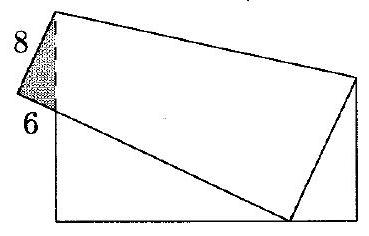
\includegraphics[max width=\textwidth, center]{2024_11_21_72654931dc1bb30ea233g-1}
\end{enumerate}

\section*{LICEUM}
\begin{enumerate}
  \item Rozwiąż nierówność
\end{enumerate}

\[
3-\log _{0,5} x-\left(\log _{0,5} x\right)^{2}-\left(\log _{0,5} x\right)^{3}-\cdots \geq 4 \log _{0,5} x
\]

\begin{enumerate}
  \setcounter{enumi}{1}
  \item Rozwiąż nierówność
\end{enumerate}

\[
\sqrt{x^{2}-16 x+64}+x \leq 7+\sqrt{x^{2}+6 x+9}
\]

\begin{enumerate}
  \setcounter{enumi}{2}
  \item Znajdź wszystkie liczby pierwsze \(p\) o tej własności, że liczba \(p+11\) jest dzielnikiem liczby \(p(p+1)(p+2)\).
\end{enumerate}

Rozwiązania należy oddać do piątku 20 listopada do godziny 10.35 koordynatorowi konkursu panu Jarosławowi Szczepaniakowi lub swojemu nauczycielowi matematyki lub przestać na adres \href{mailto:jareksz@interia.pl}{jareksz@interia.pl} do piątku 20 listopada do pótnocy.


\end{document}